% Drawing 85/05-1 -- folder 85, batch 05, archive page 87 (PDF page 88).
% Transcription: schéma remanié : sous $\gamma = \widehat{\mathbb{Z}}^{*}$ une double flèche verticale, en partie surchargée, le relie à $\gamma_0 = \mathbb{Z}^{*}$ ; sous $(\mathbb{Z}/6\mathbb{Z})^{*}$ une flèche marquée $\chi_2$ ; de $\gamma_0$ partent un long trait souligné et deux flèches obliques vers $\pm 1$, l'une barrée de gribouillis ; l'expression « $\chi_0 = \ldots$ » est surchargée
% Kind: arrow scheme between unit groups. Method 2 (schematic redraw from the facsimile). Status: partial.
% Notes: Labels as in the transcription: gamma = Z-hat* above, gamma_0 = Z* below, joined by a vertical double arrow (overwritten); a small two-headed arrow to its left; under (Z/6Z)* the arrow marked chi_2; from gamma_0 a long underlining stroke and two oblique strokes towards +-1 (one scribbled over, drawn grey). The overwritten "chi_0 = ..." is left as text in the transcription and not reproduced.
% Coordinates: 1 unit = 1 mm = 1/100 of the crop width (bbox in page fractions: [0.22, 0.52, 0.72, 0.66]).
% Redrawn by Claude (claude-opus-5-5), issue #73, 2026-11-07; not checked by a human; not compiled (no TeX in the session).
% Rights: reproduces part of the work -- behind RENDER_TRANSCRIPTS, never published by itself.
\documentclass[tikz,border=3pt]{standalone}
\usepackage{amsmath,amssymb}
\usetikzlibrary{patterns,arrows.meta}
\tikzset{pencil/.style={black!45}, struck/.style={black!35}, mark/.style={circle,draw,inner sep=1.3pt}, pt/.style={circle,fill,inner sep=0.9pt}, opt/.style={circle,draw,fill=white,inner sep=1.1pt}}
\begin{document}
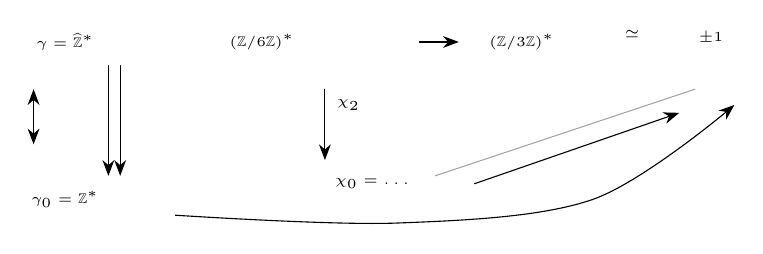
\begin{tikzpicture}[x=1mm,y=1mm,line cap=round,line join=round,font=\scriptsize]
\node[inner sep=1pt] at (8,-13) {\tiny $\gamma = \widehat{\mathbb{Z}}^{*}$};
\node[inner sep=1pt] at (8,-33) {\tiny $\gamma_0 = \mathbb{Z}^{*}$};
\node[inner sep=1pt] at (33,-13) {\tiny $(\mathbb{Z}/6\mathbb{Z})^{*}$};
\draw[-{Stealth[length=2mm]}] (53,-13) -- (58,-13);
\node[inner sep=1pt] at (66,-13) {\tiny $(\mathbb{Z}/3\mathbb{Z})^{*}$};
\node[inner sep=1pt] at (80,-12) {\tiny $\simeq$};
\node[inner sep=1pt] at (90,-12.5) {\tiny $\pm 1$};
\draw[-{Stealth[length=2mm]}] (13.5,-16) -- (13.5,-30);
\draw[-{Stealth[length=2mm]}] (15,-16) -- (15,-30);
\draw[{Stealth[length=2mm]}-{Stealth[length=2mm]}] (4,-19) -- (4,-26);
\draw[-{Stealth[length=2mm]}] (41,-19) -- (41,-28);
\node[inner sep=1pt] at (44,-21) {\tiny $\chi_2$};
\node[inner sep=1pt] at (47,-31) {\tiny $\chi_0 = \ldots$};
\draw[-{Stealth[length=2mm]}] plot[smooth, tension=0.55] coordinates {(22,-35) (50,-36) (75,-33) (93,-21)};
\draw[struck] (55,-30) -- (88,-19);
\draw[-{Stealth[length=2mm]}] (60,-31) -- (86,-22);
\end{tikzpicture}
\end{document}
